\problemname{Hectic Harbour II}

An upcycled shipping container makes a good site to open a pop-up store in a
trendy part of town. Such a business comes with its own risks -- for example,
this morning a local freight company mistook your premises for one of their
crates and sent it to the shipyard for loading.

Your crate is now sitting in the shipyard in one of two stacks ready for
loading onto the ship. Each crate except yours has its own tracking number.

\begin{figure}[h!]
  \centering
  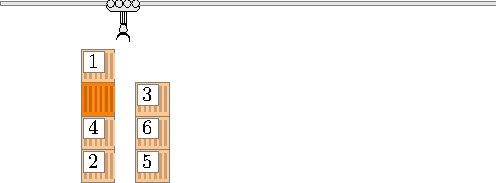
\includegraphics[width=0.8\textwidth]{sample}
  \caption{Illustration of Sample Input 2. Your business is in the unmarked crate.}
  \label{fig:crates}
\end{figure}
\vspace{-0.4cm}

The system for loading crates is automated and proceeds in a preset order.
First, the crate with the next tracking number is uncovered by picking up all of the crates on top,
one-by-one, and moving every single one across to the other stack individually.
Then the crate is taken to the ship. Since your crate is not part of this
order, it is generally ignored and will not be loaded.

After loading a crate, some time is spent securing the whole cargo on board.
This is your chance to
recover your container -- if it is on top of one of the stacks,
you will have just enough time to slide it off and get it back.

How many such opportunities will you have in total?

\section*{Input}
The input consists of:
\begin{itemize}
	\item One line with three integers
        $n$, $s_1$ and $s_2$ ($2 \leq s_1, s_2 \leq 2 \cdot 10^{5}, s_1 + s_2 = n + 1$),
        the number of crates with a tracking number, the number of crates on
        the first stack, and the number of crates on the second stack
        respectively.
	\item One line containing $s_1$ integers,
        the tracking numbers of the crates on the first stack, in order from bottom to top.
	\item One line containing $s_2$ integers,
        the tracking numbers of the crates on the second stack, in order from bottom to top.
\end{itemize}

The crates with tracking number are numbered from $1$ to $n$ and are removed
from the stacks in that order. Your crate has tracking number $0$ and will never
be on top of one of the stacks initially.

\section*{Output}
Output the number of occasions at which your crate is on top of one of the stacks and the
crane is busy loading a crate.

\begin{figure}[h!]
  \centering
  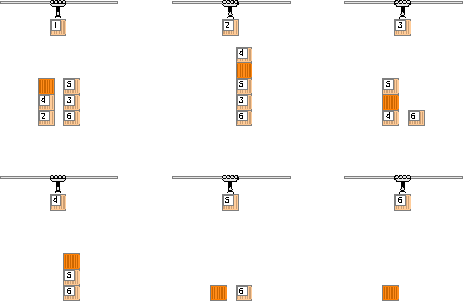
\includegraphics[width=0.8\textwidth]{harbour2/problem_statement/demo}
    \caption{Step by step illustration of Sample Input 2. There are $4$
    occasions at which your crate is on top of one of the stacks, while any of
    crates $1$, $4$, $5$ or $6$ is loaded.}
\end{figure}
